\documentclass[conference]{IEEEtran}
\usepackage{epsfig}
\usepackage[cmex10]{amsmath}
\usepackage{url}

\usepackage{multirow}
\usepackage{array}
\usepackage{footnote}

\widowpenalty=10000
\clubpenalty=10000

\begin{document}
\title{Reflection, Rendezvous, and Relaying: \\
Addressing the P2P Boostrap Problem for Small Overlay Networks}

\author{
%\IEEEauthorblockN{David Isaac Wolinsky, Pierre St. Juste, P. Oscar Boykin,
%and Renato Figueiredo}
%\IEEEauthorblockA{Advanced Computing Information Systems Lab\\
%University of Florida}
}

\maketitle

\begin{abstract}

Peer-to-Peer (P2P) overlays provide a framework for building distributed
applications consisting of few to many resources with features including
self-configuration, scalability, and resilience to node failures.  Such systems
have been successfully adopted in large-scale Internet services for content
delivery networks, file sharing, and data storage.  The bootstrap problem,
finding an existing peer in the overlay, remains a challenge to enabling these
services for small-scale P2P systems.  In large networks, the solution to the
bootstrap problem has been the use of dedicated services, though creating and
maintaining these systems requires expertise and resources, which constrain
their usefulness and make them unappealing for small-scale systems.
Decentralized, P2P systems can be useful in small-scale systems for privacy
concerns as well as supporting network applications that lack dedicated,
centralized bootstrap servers.

The novel contributions of this paper are in depth focus on the requirements
necessary for bootstrapping small-scale overlays and satisfying them through
the use of existing public overlays.  The requirements are a method for
reflection in order to obtaining a publicly reachable address, so peers behind
network address translators and firewalls can handle incoming connection
requests; rendezvous for discovering remote peers, when the overlay lacks
stable membership; and communication relaying to share public addresses and
communicate when direct communication is not feasible.  After presenting a
survey of various public overlays, we identify two overlays that match the
requirements:  XMPP overlays, such as Google Talk and Live Journal Talk, and
Brunet, a structured overlay based upon Symphony.  We have implemented
prototypes for each of these overlays and present qualitative experiences in
using them to bootstrap small-scale overlays.

\end{abstract}

\section{Introduction}

While P2P overlays provide a scalable, resilient, and self-configuring platform
for distributed applications, their adoption rate for use across the Internet
has been slow outside of large-scale systems, such as data distribution and
communication.  General use of decentralized, P2P applications targeting homes
and small/medium businesses (SMBs) has been limited in large part due to
difficulty in decentralized discovery of P2P systems, the bootstrap problem,
further inhibited by constrained network conditions due to firewalls and NATs
(network address translators).  While these environments could benefit from
P2P, many of these users lack the resources or expertise necessary to bootstrap
private~\footnote{In the context of this paper, private implies that the
overlay's purpose is not for general purpose and not that it is secure or
secret.}  P2P overlays particularly when the member state is unsteady and
across wide-area network environments where a significant amount of or all
peers may be unable to initiate direct communication with each other due to
firewalls and NATs.

Examples of large-scale P2P systems include Skype, BitTorrent, and Gnutella.
Skype is a voice over P2P system, whereas BitTorrent and Gnutella are used for
file sharing.  The bootstrapping in these systems typically rely on overlay
maintainers using high availability systems for bootstrapping, bundling their
connection information with the application for distribution.  When the
application is started, it uses these high availability servers to connect with
other peers in the system.  Alternatively, some services constantly crawl the
network and place peer lists on dedicated web sites, a new peer wishing to join
the network queries the web site and then attempts to connect to the peers on
that list.

In smaller-scale systems, interest in P2P focuses more on the decentralized
component.  Users may desire to run an application at many distributed sites,
but the application lacks dedicated central servers to provide discovery or
rendezvous service for peers.  Alternatively, dedicated, centralized P2P
service providers, such as LogMeIn's Hamachi~\cite{hamachi}, a P2P VPN, may
collect usage data, which the users may wish to remain private, or are not free
to use.  

Many applications make sense for small-scale usage including multiplayer games,
especially those that never or no longer have dedicated online services;
private data sharing; and even distributed file systems.  Clearly, a small P2P
system could be bootstrapped by one or more users of the system running on
public addresses, distributing addresses through e-mail or phone, instructing
his peers to connect to add that address to their P2P application, and then
initiate bootstrapping; but these types of situations are an exception and not
the norm.  Instead, we focus on the components that can make decentralized
bootstrapping transparent to the user, so that user interaction with the P2P
component of the application is minimal and intuitive.

\begin{figure*}[h!t!]
\centering
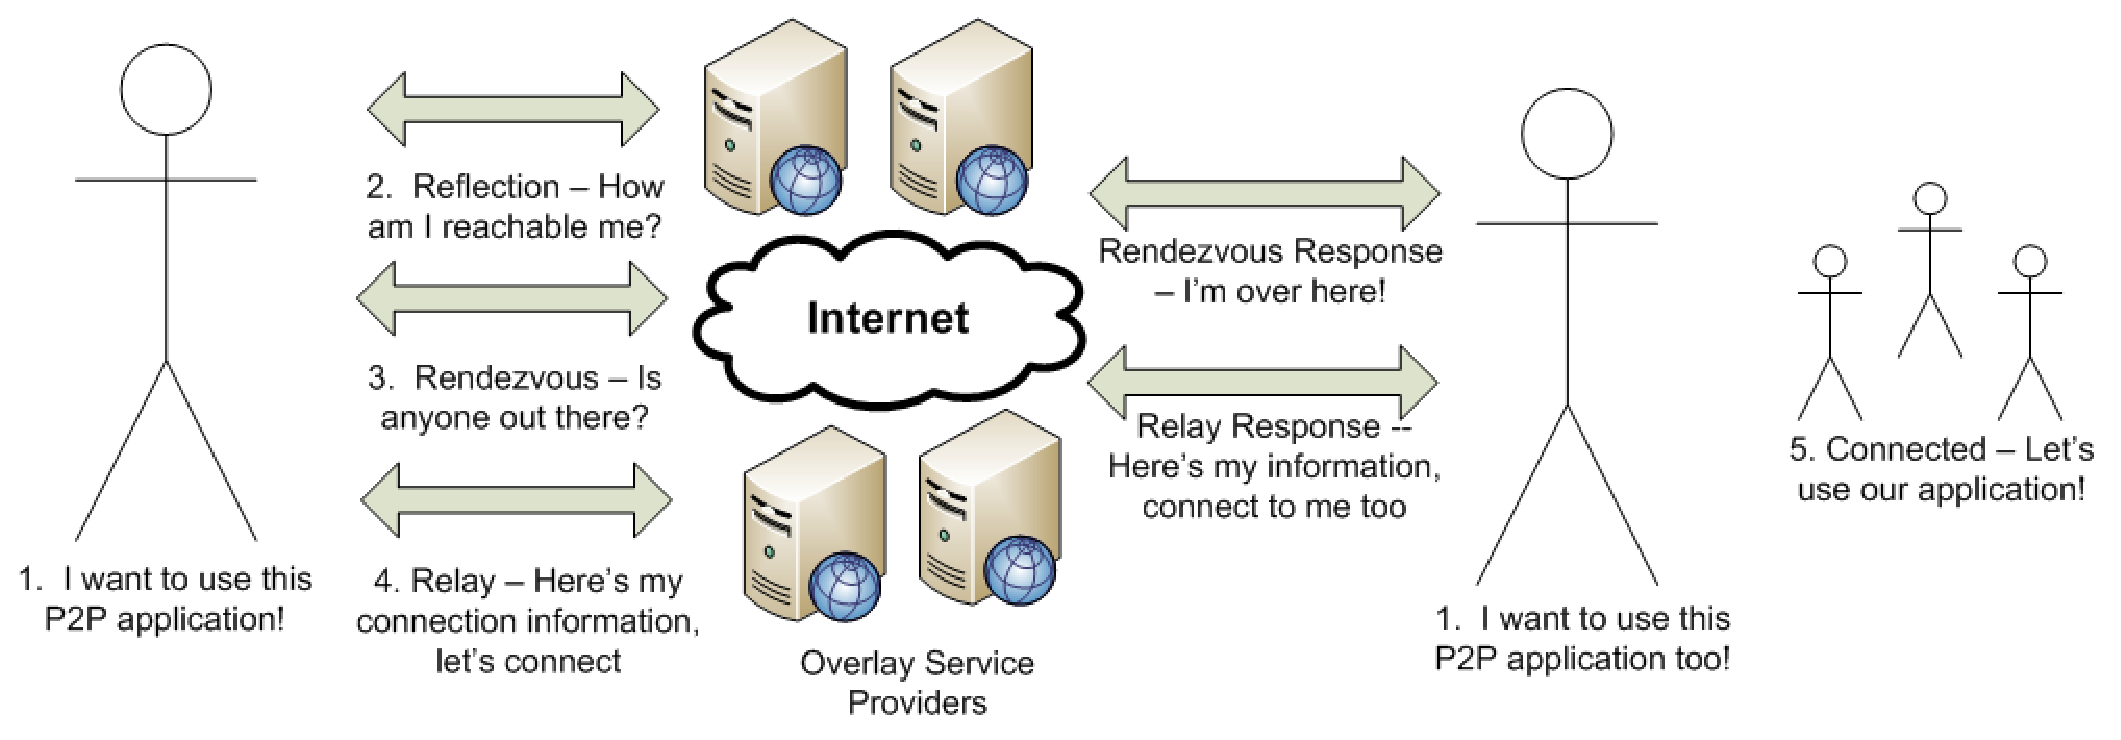
\epsfig{file=figs/bootstrap.eps, width=5.5in}
\caption{Bootstrapping a P2P system using an existing (generic) overlay.}
\label{fig:bootstrap}
\end{figure*}

The basic bootstrapping process can be broken down into two components finding
a remote peer and then successively connecting to more peers.  When a node
bootstraps into a P2P system, it contacts bootstrap servers, until it
successfully connects with one.  Upon connecting with a bootstrap server, the
two exchange information.  The bootstrap server may inquire into the overlay
for the best set of peers for the new peer and respond with that information or
it may respond with its existing neighbors.  At which point, the peer attempts
to connect with those peers.  This process continues aggressively until the
peer arrives at a steady state, either connecting with a set of specific set or
count peers.  Afterward, the P2P logic becomes passive, only reacting to churn,
that is new incoming peers or outgoing peers.

Overlay support for constrained peers, those behind NATs and restrictive
firewalls, requires additional features to support all-to-all connectivity for
peers in the overlay.  Thus the instantiation of P2P systems for private use
could become overly burdensome and rely on significant human interaction to
bootstrap them, such as relaying connection information through phone calls and
e-mail.  Even if this is feasible, this sort of interaction is undesirable, P2P
systems should be self-discovering so that users need to do minimal amount of
work to take advantage of them and adhoc systems stress this point.  In
addition, these may rely on centralized components, if they become unavailable,
which is a possibility since most users lack the expertise in configuring
highly available systems, the system will not be accessable.

To address this, we explore the use of existing public overlays as a means to
bootstrap private overlays.  There are many existing wide-spread systems with
high availability, such as Skype, Gnutella, XMPP, and BitTorrent; by leveraging
these systems, system integrators can easily enable users to seamlessly
bootstrap their own private P2P systems.  In the preceding paragraphs, we
identified the components necessary for bootstrapping a homogeneous system, now
we expand them for environments to support the bootstrapping of a private
overlay from a public overlay with consideration for network constrained peers.
The public overlay must support the following mechanisms as illustrated in
Figure~\ref{fig:bootstrap}:
\begin{enumerate}
\item \textbf{Reflection} - Constrained peers must have some method of
determining their Internet connection information, to share with other
constrained peers to enable direct connectivity.
\item \textbf{Rendezvous} - Peers seeking members of a private overlay in a
public overlay must be able to identify each other.
\item \textbf{Relaying} - Peers must be able to exchange arbitrary data to
share connection information and to enable direct links across NATs when
possible or, otherwise, as a relay.
\end{enumerate}
This work motivates from the belief that what prevents use of P2P systems is
due to lack the resources, technical knowledge, and lack of ability and desire
to create and manage high availability bootstrap services.  A public overlay
can be used to transparently bootstrap a private overlay with minimal user
interaction.

These requirements will be presented and verified in the context of two
prototype implementations: a XMPP (Jabber)~\cite{xmpp} and
Brunet~\cite{brunet}.  XMPP or Extensible Messaging and Presence Protocol based
overlays are commonly used as chat portals, for example, GoogleTalk and
Facebook Chat use the protocol.  XMPP also supports a P2P overlay amongst
servers forming a XMPP Federation allowing inter-domain communication amongst
chat peers, so that users from one XMPP server can communicate with those using
another.  Brunet provides generic P2P abstractions as well as an implementation
of the Symphony structured overlay.  We present the architecture for these
systems, the lessons learned in constructing and evaluating them,  as well as
provide quantitative analysis of peer connectivity to a private Brunet overlay.

The organization of this paper follows.  Section~\ref{background} presents
common P2P overlay technologies, motivating examples for this work, existing
solutions to the bootstrapping problem, and NAT challenges in P2P systems.  In
Section~\ref{overview}, we present a survey of overlays, applying the
requirements for private overlay bootstrapping to them, and then show in detail
how they can be applied to Brunet and XMPP.  In Section~\ref{evaluations}, we
then perform a timing evaluation of bootstrapping overlays using our prototype
running on PlanetLab.  Finally, we conclude the paper with
Section~\ref{conclusions}.

\section{Background}
\label{background}
\subsection{Common P2P Systems}

Large-scale P2P systems typically come in two flavors:  unstructured and
structured.  Unstructured systems~\cite{gnutella, fasttrack} are generally
constructed by peers attempting to maintain a certain amount of connections to
other peers in the P2P system, whereas structured systems organize into
well-defined topologies, such as trees, 1-D rings, or hypercubes.  Though
unstructured systems are typically simpler to bootstrap and maintain, they rely
on global knowledge, flooding, or stochastic techniques to search for
information in an overlay and thus creating potential scalability constraints.
Alternatively, structured systems~\cite{pastry, chord, symphony, kademlia,
can}.  have guaranteed search time typically with a lower bound of $O(\log N)$,
though recent research has shown that these systems can be constructed to
support $O(1)$ search time~\cite{beehive}.

A key component of most structured overlays is support for decentralized
storage / retrieval of information by mapping keys to specific node IDs in an
overlay called a distributed hash table (DHT).  At a minimum, the data is
stored at the node ID either smaller or larger to the data's node ID and for
fault tolerance the data can be stored at other nodes.  DHTs can be used by
peers of systems to coordinate allocation and discovery of resources, making
them attractive for self-configuration in decentralized collaborative
environments.

Another subset found in various scale environments are ``P2P'' systems that are
not fully decentralized, such as ``P2P VPNs'' like Hamachi~\cite{hamachi},
older systems like the original Napster, and tracker-based BitTorrent.  These
types of systems provide a rendezvous services for peers to discover each other
to form direct, or P2P, connections with each other for the purpose of network
connectivity or data sharing.  BitTorrent differentiates itself by using the
trackers as a gateway into the overlay, once inside, peers exchange connection
information with each other directly relegating the tracker as a fall back.
This approach has enabled BitTorrent to be modified to support trackerless
torrents through using a DHT.

\subsection{Applications}

In this section, we present applications and potential ways to configure them
to use a private overlay.  The work relies on a public key infrastructure and
secure point-to-point and end-to-end communication for P2P as described in our
technical report~\cite{vpo}.  The applications we investigate include chat
rooms, social networks, VPNs, and multicast.  The key to all these applications
is that users can easily host their own services and be discovered through the
use of a free-to-join public overlay.

\subsubsection{Chat Rooms}

Chat rooms provide a platform for individuals with a common interest to find
each other, group discussion, private chat, and data exchange.  One of the most
popular chat systems for the Internet is Internet Relay Chat (IRC).  As
described in~\cite{irc}, IRC supports a distributed tree system, where clients
connect to a server, and servers use a mixture of unicast and multicast to
distribute messages.  The issues with IRC are documented by~\cite{irc_arch},
namely, scalability due to all servers needing global knowledge, reliability
due to connectivity issues between servers, and lack of privacy.  Private
overlays could be extended to support the features of IRC and potentially deal
with these inherent issues.  Each chat room would be mapped to a private
overlay and the public overlay would be used as a directory to learn about
available chat rooms and request access.  Structured overlays could easily be
used as servers for IRC, do not require global knowledge, and can be configured
to handle connectivity issues.

\subsubsection{Social Networks}

Social networks such as Facebook and MySpace provide an opportunity for users
to indirectly share information with friends, family, and peers via a profile
containing personal information, status updates, and pictures.  Most social
network structures rely on hosted systems, where they become the keepers of
user data, which creates privacy and trust concerns.  Private overlays can
remove this third party, making users the only owner of their data.  For this
model, we propose that each user's profile be represented by a private overlay
consisting of their friends.  The overlay should include a secured DHT, where
only all writes are signed to uniquely identify the creator and may only be
removed by the owner of the overlay.  In addition to bootstrapping the private
overlays, the public overlay would be used as a directory for users to find and
befriend each other.  For fault tolerance and scalability, each user provides a
copy of their profile locally, which will be distributed amongst the private
overlay in a read-only DHT, therefore, allowing the user's profile to be
visible whether they are offline or online.  Each user's social network would
than consist of the accumulation of the individual private overlays and the
public overlay.

\subsubsection{P2P VPNs}

Private overlays enable truly decentralized, P2P VPNs.  The most common type of
VPNs are centralized VPNs like OpenVPN, which requires that a centralized set
of resources handle session initialization and communication.  Another approach
taken by Hamachi and many others is to maintain a central server for session
initialization but allow communication to occur directly between peers and
providing a central relay when NAT traversal fails.  SocialVPN~\cite{socialvpn}
relies on a dedicated bootstrap overlay provided by University of Florida.
Using the techniques described in this paper, SocialVPN could be extended so
that it can be bootstrapped into private systems without additional user
configuration.

\subsubsection{Multicast}

The topic of secure multicast has been a focus of much research.  Using an
approach similar to CAN~\cite{can_multicast}, a virtual private overlay forms a
ring where all nodes are members of the multicast group with the additional
feature that you can trust that your audience is limited to those in the
overlay.  The main advantage of such multicasting technologies would be for
wide-area, distributed multicast as described in~\cite{from_peer}.  Examples of
such services include light weight multicast DNS / DNS-SD (service discovery),
as well as audio and video streaming.

\subsection{Bootstrapping P2P Systems}

As described in the introduction, the simple case of bootstrapping is limited
to one peer attempting to find an active peer in the overlay in order for
itself to become a member.  The large-scale providers have resources not
readily available to small-scale overlays.  This section presents the existing
techniques and those being developed and describes their application to
susubbsmall-scale systems.

When using dedicated bootstraps, a service provider hosts one or more bootstrap
resources.  Peers desiring to join the overlay query the bootstrap nodes, until
a successful connection is made to one.  The bootstrap server will then assist
in connecting to other nodes in the P2P system.  The bootstrap nodes are either
packaged with the application at distribution time or through a meta data file,
such as in BitTorrent.  In small, ad hoc pools, draw backs to this approach are
the same server would have to be used every time to bootstrap the system or
users would have to reconfigure their software to connect to new bootstrap
servers over time.  A bootstrap server creates a single point of failure,
especially when not being deployed using high availability techniques.  This
approach requires at least one peer to have a publicly accessible address.

Another commonly used approach for large-scale systems is the use of a host
cache~\cite{host_cache}.  Clients post current connection information to
dedicated web services, a host cache, that cache the connection information and
URLs to other host caches.  For small, ad hoc networks, a host cache acts no
differently than a centralized rendezvous point, requiring that at least one
peer has a publicly accessible address.

A similar concept to host caches is used by the ``P2P VPN''~\cite{p2pvpn} using
a BitTorrent tracker.  In this process, one user registers a file via the hash
of it to a centralized tracker.  In the ``P2P VPN'', this was not a file, but
rather a unique identifier for the VPN.  Peers register with the tracker their
IP address and are able to receive other active users IP addresses.  Peers on
public addresses, not behind NATs or firewalls, are able to receive incoming
connections from all other peers.  The problem with this approach is that it is
heavily use driven.  A user must register with each BitTorrent tracker
individually and maintain a connection with each of them, in order to handle
cases where BitTorrent trackers go offline.  In addition, this does not use the
BitTorrent trackers in a normal fashion, so it may be banned by tracker hosts.

Research has shown that peers can use the locality properties of recent IP
addresses in a large-scale P2P system can be used to make intelligent guesses
about other peers in the P2P system in an approach called random
probing~\cite{bootstrapping_p2p, locality_aware}.  The results show for
networks in the order of tens of thousands that a peer can find an active peer
node within as few as 100 attempts and as many as 2,000 guesses.  The
application of this approach to small, ad hoc groups is challenging.  If peers
are behind NATs, the port mapping may change randomly or not be the same for
multiple peers, further more, if peers are widely distributed and very small,
this approach may have to query the majority of the IP address range to find a
peer.  Additionally, the approach assumes that all peers were on public
addresses and that each used a constant port to host the P2P application.  The
results were not tested in real systems, but instead using overlay traces.

Rather than distribute an IP address, which points explicitly to some location
in the Internet, a small P2P network can apply a name abstraction around one
peer in the overlay using Dynamic DNS~\cite{bootstrapping_ddns}.  In this
approach, peers share a common DNS entry, providing a common means to bootstrap
the overlay.  When the peers detect that the IP directed to by the host is
offline, they use a random time back off algorithm to replace it.  The
application of this approach to small, ad hoc groups is actually quite nice, as
the service could be distributed across multiple Dynamic DNS registrations.
The significant drawback to the approach is that the dynamic DNS server could
be attacked, since the login information must be shared amongst all peers in
the overlay.  Also the approach requires that at least one peer be publicly
addressable and know that it is, if a non-publicly addressable peer updates the
cache, it could delay or permanently prevent peers from creating a P2P system.
The results were simulation based and did not determine how well a dynamic DNS
handles rapid changing of name to IP mappings.

IP supports multicasting to groups interested in a common service.  In the case
of bootstrapping a P2P system~\cite{pastry, locality_aware}, all peers would be
members of a specific group.  When a new peer comes online, it would query this
group for connection information and then connect to those that respond.  The
drawback to this approach is that it only works in environments connected by IP
multicast, typically local area networks only, thus for a wide-area,
distributed P2P system, this approach will most likely not work.

A large-scale structured overlay~\cite{one_ring, p2p_bootstrap} could enable
peers to publish their information into a dedicated location for their service
or application and then query that list to obtain a list of online peers.
Peers could then come online, search for peers in their overlay, and then
connect with them using their connection information.  Since the service would
be a large-scale system, it could easily be bootstrapped by a dedicated
bootstrap or host caches.  As it stands, the described works were position
papers and the systems have not been fully fleshed out.  The primary challenge
in relationship to small, ad hoc networks is that it lacks details
bootstrapping of peers behind NATs into overlays as it provides only a means
for rendezvous and no reflection nor relaying.

\subsection{Network Address Translation Hampering the Bootstrap Process}

As of 2010, the majority of the Internet is connected via Internet Protocol
(IP) version 4.  This protocol has a quickly approached limit of addresses
available,  only $2^{32}$ (approximately 4 billion).  With the Earth's
population at over 8 billion and each individual potentially having multiple
devices with Internet connectivity, the IPv4 limitation is becoming more and
more apparent.  Addressing this issue are two approaches:  1) the use of NATs
to enable many machines and devices to share a single IP address but preventing
bidirectional connection initiation, and 2) IPv6 which supports $2^{128}$
addresses.  The use of NATs complicates the bootstrapping of P2P systems as it
prevents peers from simply exchanging addresses with each other to form
connections, as the addresses may not be public.  In addition, firewalls may
prevent peers from receiving incoming connections.  Thus while the eventual
widespread use IPv6 will cause the demise of NATs, though this is not
guaranteed, it does not deal with the issue of firewalls preventing P2P
applications from communicating.

When a machine, \textit{A}, behind a typical NAT, \textit{B}, sends out a
packet to an Internet host, \textit{C}, the NAT device translates the packet so
that it appears it is coming from the NAT device.  The packet sent from
\textit{A} to \textit{C} has the source and destination $IP:port$ pairs
expressed as $IP_A:Port_A$ and $IP_C:Port_C$, respectively.  \textit{A}
forwards the packet to \textit{B} who transforms the source from $IP_A:Port_A$
to $IP_B:Port_B$, where $Port_A$ may or may not be equal to $Port_B$.  This
creates a NAT mapping so that incoming packets from $IP_C:Port_C$ to
$IP_B:Port_B$ are translated and forwarded to $IP_A:Port_A$.

There are a handful of recognized NAT devices as presented in~\cite{stun,
p2p_nats_rfc}.  The following list focuses on the more prevalent types:
\begin{itemize}
\item \textbf{Full cone} - All requests from the same internal IP and port are
mapped to a static external IP and port, thus any external host can communicate
with the internal host once a mapping has been made.
\item \textbf{Restricted cone} - Like a full cone, but it requires that the
internal host has sent a message to the external host before the NAT will pass
the packets.
\item \textbf{Port restricted cone} - Like a restricted cone, but it requires
that the internal host has sent the packet to the external hosts specific port,
before the NAT will pass packets.
\item \textbf{Symmetric} - Each source and destination pair have no relation,
thus only a machine receiving a message from an internal host can send a
message back.
\end{itemize}

Peers on cone NATs can easily establish direct communication links through a
process of NAT hole punching, so long as a third-party assists in determining
the port allocated, STUN~\cite{stun_rfc}, by the NAT and another acts as a
medium for the peers to exchange this information.  Peers behind symmetric NATs
cannot easily communicate with each other, since there is no relation between
remote hosts and ports and local ports.  Further complicating the matter is
that there are various types of symmetric NATs, having behaviors similar to
full, restricted, and port restricted cone NATs.  \cite{ice} describes methods
to traverse these NATs so long as there is a predictable pattern to port
selection.  Approaches that that use hole punching generally use UDP.  UDP,
unlike TCP, lacks state, thus traversal attempts do not need to be concerned
with potentially replaying message, limitations of the socket libraries, or
handling potential reject methods that may occur when attempting to perform TCP
hole punching;  though there is reasonable amount of work describing TCP NAT
traversal such as~\cite{tcp_nat}.  TCP NAT traversal is complicated by stateful
firewalls, or those that watch connections and connection attempts preventing
messages from closed TCP channels from passing through the NAT.  For situations
in which both peers are behind NATs and firewalls that prevent inbound
communication inhibiting NAT traversal, a third-party can act as a relay
between the two, known as triangulation or TURN~\cite{turn} (traversal using
relay NAT).

These NAT traversal services in themselves only deal with a small portion of
the bootstrap problem, reflection.  That is, peers are able to obtain a public
address for receiving incoming connections.  These services provide no means
for users to exchange addresses with each other.  To address this issue many
systems incorporate these NAT traversal libraries and use intermediaries to
exchange addresses.  In order for peers to form direct connections, peers still
need a mechanism to discover each other or rendezvous and then a relay pathway
to exchange their network information.

An example of an application that uses these types of services combines with
rendezvous and relay is Teredo~\cite{teredo}.  Teredo enables all peers to have
a globally identifiable IPv6 address.  The IPv6 address maps to a specific
Teredo gateway, client pair.  When two peers using Teredo attempt to connect
with each other, the Teredo servers exchange the clients IP information
obtained using a STUN-like procedure.  While this gives users a public address,
it does not do so in a scalable or fault tolerant way.  If the Teredo gateway
goes offline or becomes saturated, the peers outgoing and incoming requests may
be ignored.

\section{Bootstrapping Private Overlays}
\label{overview}

As presented in the preceding sections, a solution to bootstrapping small P2P
overlays must address several challenges, namely reflection, rendezvous, and
relaying.  In this section, we present a generic solution to this problem.  At
the basis of our solution is the use of a publicly available free-to-join
public overlay.  In order to support these features the public overlay must
have mechanisms for peers to determine their network identity and maintain
these mappings, reflection; search for other peers that are bootstrapping the
same P2P service, rendezvous; and send messages to peers through the overlay,
relaying.  These are the minimum requirements to bootstrap a decentralized, P2P
system when all peers are behind NATs.  

Without a \textbf{reflection} utility, two peers would be unable to communicate
directly with each other, when they exchange connection information, they would
only be able to share local networking information.  If they are not on the
same network, the information will be useless.  Furthermore, if they are on the
same network, then an approach using multicast would be sufficient.  Thus
assuming that the other two capabilities are available, rendezvous and
relaying, peers would only be able to communicate through the overlay, which
may introduce significant latency and bandwidth overheads.  

A system, lacking the ability to exchange messages via the overlay or
\textbf{relaying}, could limit the types of NATs peers could traverse.
Assuming reflection and rendezvous, a peer could obtain connection information
for another peer through an entry in the DHT, much like Tracker-less torrents,
and connect to it so long as the peer is either on a public address, behind a
cone NAT, or have a TURN connection, though a TURN connection would violate the
expectation of the overlay lacking relay capabilities.  In other all other NAT
cases, a peer must initiate simultaneous connection attempts in order to form a
direct connection.  Furthermore, while TURN may provide relaying, it is not
very scalable unless the features is built decentrally into the overlay.

Without \textbf{rendezvous}, peers would have no mechanisms to discover each
other, in this case, random probing would be the only mechanism for peers to
discover each other.  If the peers are behind NATs, not even random probing
would be sufficient for them to form connections with each other.  Thus
rendezvous is the most important component without it, peers would be unable to
find each other.

\begin{table*}[h!t!]
\centering
\begin{tabular}[c]{|m{1.5cm}||m{5.5cm}|m{3cm}|m{3cm}|m{3cm}|}
\hline & Description & Reflection & Rendezvous & Relay \\ \hline \hline
BitTorrent &
Basic BitTorrent systems rely on a centralized tracker to provide the initial
bootstrapping.  At which point, the peers no longer require use of the tracker,
but it can be used to monitor the state of the file distribution and ensure
good distribution of file providers, seeds.  BitTorrent specifies a protocol,
though each client may support additional features not covered by the protocol.
&
In general, the current specification does not support NAT traversal, though
future versions may potentially use UDP NAT traversal.  At which point,
BitTorrent may support a reflection service.
&
As mentioned in the previous section, peers can register as seeds to the same
file hash, thus their IP address will be stored with the tracker.
&
Peers receive each other's IP addresses from the tracker, and there is no
inherent relaying.
\\ \hline
Gnutella &
Gnutella is a large-scale unstructured overlay, consisting of over a million
active peers.  Gnutella's is primarily used for file sharing.  Skypes general
make up consists of a couple thousand super, ultra, peers to provide
reliability to the overlay.  Gnutella is free-to-join and requires no
registration to use.
&
Work in progress.  Peers attempt to connect to a sharers resource, though a
"Push" notification reverses this behavior.  Thus a peer behind a NAT can
share with a peer on a public address.
&
Peers can perform broadcast searches with TTL up to 2, when networks consist of
millions of peers, small overlays will most likely not be able to discover each
other.
&
Not explicitly, could potentially utilize ping messages to exchange messages.
\\ \hline
Skype &
Skype is a large-scale unstructured overlay, consisting of over a million
active peers.  Skype is primarily used for voice over P2P communication.
Skype, like Gnutella, also has super peers, though the owners of Skype
provides authentication and bootstrap servers.  Though Skype is free-to-join,
it requires registration to use.
&
Skype APIs provide no means for reflection.
&
Skype allows extensions through applications.  It is possible for peers to
broadcast queries to each other, transparently from the user, to determine if
a given user has an application installed.  Thus Skype does support rendezvous.
&
Skype applications are allowed to route messages via the Skype overlay, but
because Skype lacks reflection, all communication must traverse the Skype
overlay.
\\ \hline
XMPP &
XMPP consists of a federation of distributed servers.  Peers must register
an account with server, though registration can be done through XMPP APIs
without user interaction.  XMPP is not a traditional P2P system, though it
has some P2P features.  XMPP servers allow peers on distinct XMPP servers
to communicate with each other.  The links between servers are created
based upon client demand.  The links are trusted due to a certificate
provided, when the server joins the XMPP Federation.
&
While not provided by all XMPP servers, there exist extensions for NAT
traversal.  GoogleTalk, for example, provides both STUN and TURN servers.
&
Similar to Skype, XMPP friends can broadcast queries to each other to find
other peers using the same P2P service.  THus XMPP supports rendezvous.
&
The XMPP specification allows peers to exchange abitrary out of band
communication with each other.  Most servers support this behavior, even
when sent across the Federation.  Thus XMPP supports relaying.
\\ \hline
Kademlia~\cite{kademlia} &
There exists two popular Kademlia systems, one used by many BitTorrent systems
and the other used by Gnutella, called Mojito.  Kademlia implements an
iterative structured overlays, where peers query each other directly when
searching the overlay.  Thus all resources of a Kademlia overlay must be
publicly addressable.
&
Existing implementations of Kademlia does not support mechanims for peers to
determine their network identity.
&
Peers can use the DHT as a rendezvous service, storing their connectivity
information in the DHT at key location:  $hash(SERVICE)$.
&
An iterative structured overlay has no support for relaying messages.
\\ \hline
OpenDHT~\cite{opendht} &
OpenDHT was until recently a freely available DHT running on PlanetLab, though
it was  recently decommissioned.  OpenDHT is built using Bamboo, a Pastry-like
protocol~\cite{pastry}.  Pastry implements recursive routing, where peers
in the overlay forward messages for each other from source to destination.
&
Existing implementations of Bamboo and Pastry do not support mechanims for
peers to determine their network identity.  Though this is ongoing work.
&
Peers can use the DHT as a rendezvous service, storing their connectivity
information in the DHT at key location:  $hash(SERVICE)$.
&
Because Pastry uses recursive routing, it can be used as a relay.  Furthermore,
extensions to Pastry have enabled explicit relays called virtual
connections~\cite{epost}.
\\ \hline
Brunet~\cite{brunet} &
Brunet like OpenDHT is a freely available DHT running on PlanetLab, though
still in active development.  Brunet creates a Symphony~\cite{symphony} overlay
using recursive routing.
&
Brunet supports inherent reflection services, when a peer forms a connection
with a remote peer, the peers exchange their view of the relationship.
&
Peers can use the DHT as a rendezvous service, storing their connectivity
information in the DHT at key location:  $hash(SERVICE)$.
&
Like Pastry, Brunet supports recursive routing and even supports relays called
tunnels~\cite{hpdc08_0}.
\\ \hline
\end{tabular}
\caption{}
\label{tab:overlays}
\end{table*}

Table~\ref{tab:overlays} reviews various overlays, the majority of which are
public free-to-join overlays, though some research only overlays are included.
The overlays were chosen based upon their scale and availability.  From this
the most attractive two services are Brunet and XMPP.  Brunet provides
traditional P2P infrastructure, though lacks the large-scale and high
availability features due to being rooted in an academic project.  XMPP,
on the other hand, is a non-traditional overlay and limits private overlays
to being bootstrapped through friendship connections.  While most users
seeking a private overlay will do so with friends, this may not always be the
case, consider video game players searching for people to play with online.
On the other hand, XMPP is built on top of production systems thus has
more applicability to real world usage.

A single public overlay does not need to provide all the components for
bootstrapping the private overlay.  For example, peers could use the the
Limewire / Gnutella Kademlia DHT, Mojito, as a means to register for
rendezvous.  The peer could leave their globally unique XMPP identity in the
DHT.  Another peer interested in the same service would discover this identity
and then could become friends through XMPP, an automatable process.  Once the
friendship has been formed, they can use XMPP as a means for relaying.

\subsection{Bootstrapping Private Overlays Using Brunet}
\label{brunet_bootstrapping}

As mentioned earlier, Brunet, based upon the Symphony structured P2P overlay,
is a freely available P2P library, supporting STUN and TURN-like NAT traversal.
In this section, we describe how one could use a public Brunet overlay to
bootstrap private overlays.  

Brunet bootstraps using dedicated bootstrap services, though each peer can
support a bootstrap list of 10,000 potential bootstrap nodes.  With every
connection Brunet makes, peers inform each other of their view of the remote
peers network state, in other words, a form of passive \textbf{reflection}.
When a peer attempts to connect to another, they route ``ConnectToMe'' messages
across the overlay informing of the remote peer of the desire to connect.  This
message causes the peers to exchange their network information and both peers
attempt to form connections simultaneously.  This approach of bootstrapping
handles all forms of NATs besides those that fall under symmetric and firewalls
that prevent UDP.  To address these types of NATs, Brunet also supports forming
``Tunnels''~\cite{hpdc08_0}, where peers exchange near neighbor information.
If there exists overlap, then a connection will form.  As presented in their
work, the probability of overlap for overlay required connections, peers near
each other in the overlay address space.

The approach for \textbf{rendezvous} in a DHT follows.  All peers interested in
a specific service or private overlay obtain a DHT key based upon a hashing of
the service' or private overlay's name.  Peers can then query this entry in the
DHT to obtain a list of peers in the private overlay.  Note, that Brunet's DHT
implementation supports a single key may have many values.  Since DHTs are soft
state, or lease systems, where data is released after a certain period of time.
Peers must actively maintain their DHT entry.  

The data stored in the DHT is the peers public overlay address.  Doing this
enables a peer to use the Brunet overlay for \textbf{relaying}, we call this a
``Subring'' transport.  This requires that peers remain actively connected to
the public overlay, so long as they are members of the private overlay,
otherwise the peers could not use the service for relaying.

In order to take advantage of Brunet's reflection service for the private
overlay, we use a technique for multiplexing transports called ``Pathing''.
Pathing works by wrapping a multiplexing system around an underlying transport
mechanism, such as UDP or TCP.  As an example, when two peers desire to have
communication with each other, they exchange end point information.  In a
system without Pathing, this would be IP addresses and port numbers.  Pathing
extends this to include a URI (universal resource identifier) path, like
``udp://192.168.1.1:15222/path''.  The Pathing transport recognizes the path as
belonging to one of the various overlays and forwards it to the appropriate
listener.  By using the same sockets and bindings as the public overlay peer, a
private overlay peer has access to the public overlays reflection service.
This requirement means that in order to properly take advantage of Brunet
reflection without significant code modification to Brunet, peers would need to
reuse the Brunet's transport library.

The node should maintain membership in the public overlay when connected with
the private overlay.  This is needed for two reasons: first, so that other
peers can discover the node while following the same set of steps; and second,
for NAT traversal purposes, as discussed in the next paragraph.  Because the
public overlay and its DHT provides a means for discovery, nodes must maintain
their node ID in the public overlay's DHT.  A data inserter must constantly
update the lease for the data object, otherwise the data will be removed, due
to the soft state or leasing nature of DHT, whereupon (key, value) pairs are
removed after a lease has expired.

\subsection{Bootstrapping Private Overlays Using XMPP}
\label{xmpp_bootstrapping}

The key features that make XMPP attractive are the distributed nature of the
federation and the openness of the protocol.  As of December 2009, there are
over 70 active XMPP servers in the XMPP Federation~\cite{xmpp_servers}.  These
include GoogleTalk, Jabber.org, and Live Journal Talk.  Even recently Facebook
Chat deployed XMPP capabilities.  Though unfortunately, the Facebook
implementation is incomplete acting as a proxy into their private chat servers
and thus providing only a limited subset of the XMPP features.

In XMPP, each user connects to a single XMPP service provider and maintains
this single connection for the lifetime of the application.  Messages between
users are routed through this server and the XMPP Federation.  Each user in the
XMPP has a unique identifier of the form ``username@domain''.  For two users in
the same domain, the domain name makes for little consequence.  Though when two
users are in separate domains, the XMPP servers for those domains register with
each other to proxy messages for the two users as well as other pairs that have
an active XMPP relationship.  When a user sends another user a message, it is
encapsulated in XML, the destination is set to the remote peer, and it is sent
to the server.  The server relays the packet to the destination.  Similary,
when two peers are on separate domains, the server takes the domain portion of
the user identifier and forwards it to that XMPP server, which will then relay
the message to the destination peer.

To differentiate amongst multiple sessions, each instance of a XMPP client a
user has logged in receives or sets a resource identifier, this is appended to
the user identifier represented by ``username@domain/resource''.  Thus two peers
can explicitly state the destination XMPP client instance for outgoing
messages.

Peer relationships are maintained by the server, though peers initiate them
through a subscription mechanism.  One peer requests to subscribe to the other,
and the other can either accept or deny.  The process is performed through an
XMPP client using an XMPP query service.  Once two peers have subscribed to
each other, they are notified when an instance of each others XMPP client comes
online.  These are called presence notifications.  The presence notification
provides users the state of the XMPP client and its complete user identifier,
including user name, domain, and resource.

The final baseline feature of XMPP is the XMPP query service.  Peers can send
to the server and each other ``IQ'' messages, which are control messages that
are transparent to the user.  An example of an IQ is the subscription messages
used to establish a friendship.  The use of IQs enables XMPP to be extensible,
peers that support or implement an extension respond with a positive result and
those that do not return a negative.  Recent work by Google engineers has used
the IQ to implement discovery of STUN and TURN servers called
``Jingle''~\cite{jingle}.  These features are provided free of charge through
GoogleTalk.  Peers use these services for \textbf{reflection} to obtain public
addresses.

\textbf{Rendezvous} in XMPP takes advantage of the resource portion of the user
identifier.  If the base portion of the resource string matches what the peer
is seeking, it has found a peer seeking the same service.  For example, common
resource strings are ``BitlBeeABC1234'' or ``P2P.CDEFABC''.  Thus a peer
seeking a P2P service would be under the impression that the node
``P2P.CDEFABC'' is also.  The node would then \textbf{relay} an IQ through the
XMPP server to verify this, exchange network configuration information, and
initiate connection bootstrapping.

\section{Evaluating Overlay Bootstrapping}
\label{evaluations}
In this section, we describe our prototype implementation, the experimental
setup and results, and some experiences of our experiences from deploying
overlays using XMPP.

\subsection{Our Implementation}

Our implementation makes heavy use of the transports library provided by
Brunet~\cite{brunet}.  We have extended the Brunet transports library to allow
for sending messages between peers in one overlay to another overlay as well as
an XMPP overlay.  The XMPP library we used is called Jabber-Net.  Each
connection between peers is uniquely identified by employing socket like
concepts, i.e., a pair of addresses and ports.  The basic representation for
this constitutes a pair of identifiers of the form ``brunet://P2P\_ID:PORT'',
where each peer has a unique ID and port associated for the local and remote
entity.  The XMPP implementation has a similar format:
``xmpp://USERNAME@DOMAIN:PORT/RESOURCE'', again one identifier for the local
peer and one for the remote.

For evaluation purposes, we reused the Brunet structured overlay service to
construct a private P2P overlay.  Using a structured overlay may seem strange
in such a small environment, though it actually applies quite cleanly.  In
small networks, several structured overlays act as $O(1)$ systems, this
includes Brunet and Pastry.  This value is configurable at run time, enabling
systems to support form all-to-all connectivity with peers without user
intervention.  A structured overlay applies unique identifiers to each peer and
in the case that two peers are not directly connected, greedy routing methods
can be used to route messages to each other.  Unlike unstructured systems,
which may require that the peers know the structure of the entire system or use
stochastic techniques to route packets between each other.

\subsection{Deployment Experiments}

The purpose of our experiment is to verify that our techniques work and what
overheads should be expected in using Brunet and XMPP to bootstrap an overlay.
The experiments in no means are rigorous as that would become overly focused on
overheads of Brunet and XMPP, instead this paper is primarily interested in
forming small-scale overlays.  The experiment represents 5 peers desiring
all-to-all direct connectivity a feature transparently available to them if
they bootstrap into a private Brunet overlay.

This experiment relied on a public Brunet overlay consisting of over 600 nodes
running on PlanetLab.  PlanetLab~\cite{planetlab} is a consortium of research
institutes sharing hundreds of globally distributed network and computing
resources.  PlanetLab provides a very interesting environment as there is
constant unexpected churn of machines due to the extreme load placed on the
resources and unscheduled system restarts.  Complementary to simulation,
PlanetLab gives us a glimpse of what to expect from the P2P software stack when
used in an actual environment subject to higher variance due to resource
contention and churn.

GoogleTalk provided the XMPP overlay used in this experiment.  Though this
experiment does not take into advantage the features of the XMPP Federation,
this aspect is presented in more detail in the next section reviewing
experiences deploying overlays using XMPP.

\subsection{Deployment Experiences}

In this section, we share some our experiences in deploying XMPP overlays.
Recently, Facebook announced that they would be supporting XMPP as a means to
connect into Facebook chat.  This was rather exciting and further motivated
this work, as Facebook has over 400 million active users, which would have made
there XMPP overlay, potentially, the largest free-to-join overlay.
Unfortunately, experiments established that Facebook does not actually employ a
traditional XMPP setup.  The Facebook XMPP setup merely provides a proxy into
their chat network, preventing features like arbitrary IQs and other forms of
out-of-band messages to be exchanged between peers.  That alone was not the
nail in the coffin, as messages could have still been exchanged encoding the
binary data as text messages between peers.  The nail in the coffin was that
translation performed on peers identifiers.  For example, a user would generate
a XMPP identifier of the form ``username@chat.facebook.com/resource'', but to
its peers, it would be presented as ``uSOME\_NUMBER@chat.facebook.com''.  Thus
peers would then need to use another service just to obtain the identity of the
peer and would have no means to tell what the resource identifier is.  The only
approach to bootstrapping would be to broadcast in-band messages to all peers,
the problem with this is that many peers may actually be using the chat system
for chatting.  These peers would receive spam from an overlay bootstrap, which
they may not be very receptive to.  Finally, Facebook is not a part of the XMPP
Federation, thus peers from GoogleTalk cannot chat with peers from Facebook.
Given that there was no way to exchange arbitrary information and the
rendezvous service was crippled, at this point in time, it appears there is no
way to bootstrap an overlay using Facebook.

During initial tests in verifying the workings of the XMPP code base, we
bootstrapped a  private Brunet overlay on PlanetLab through various XMPP
service providers.  Interestingly, GoogleTalk servers seem to ignore machines
on PlanetLab.  Using another provider, the service appeared to crash after 257
instances of the same account were online.  Unfortunately, the provider had no
contact information available, so we were unable to determine if our test
caused the crash.  There was one server that appeared have no trouble hosting
600 concurrent instances of a single XMPP user, ``jabber.rootbash.com''.  The
nodes were able to rendezvous and relay through \textit{rootbash} and form a
connected P2P system.  The setup did not require reflection, as PlanetLab
resources all have public IP addresses.

Once the system was running on PlanetLab, more tests were performed to
determine the ability to bootstrap across the XMPP Federation.  We formed
friendships, or subscriptions, between users across a few different XMPP
service providers.  In the most evaluated case, a single peer on GoogleTalk and
the PlanetLab system using \textit{rootbash}, the GoogleTalk peer would not
always receive presence notifications for all peers online, though always would
receive some.  When a peer began the relaying mechanism, itr would broadcast to
every peer, it rendezvoused or discovered.  When performing this between
GoogleTalk and \textit{rootbash}, the GoogleTalk peer would not receive a
response.  Though in reducing the broadcast to a random selection of 10 peers,
every 10 seconds until the GoogleTalk peer was connected, the peer received
responses.  The behavior indicates that the XMPP servers may have been
filtering to prevent denial of service attacks.  One last note, when
bootstrapping a peer from GoogleTalk into the \textit{rootbash} system, it
always took 1 minute for the node to become fully connected to the private
overlay.  When the peer used \textit{rootbash}, the peer always connected
within 30 seconds.  It seems as if the communication between XMPP servers was
being delayed for some reason.  The same behavior was not experienced, when
chatting between the two peers.

\section{Conclusion}
\label{conclusions}

In this paper, we have established the requirements for bootstrapping small-scale
P2P overlays, reflection, rendezvous, and relaying.  Reflection is required, so
that peers behind NATs and firewalls can obtain a public address to share with
remote peers.  Rendezvous is a common problem, even for large-scale systems,
peers must have a mechanism to find other peers connecting to are are in the
same overlay.  Finally, without relaying, peers behind NATs would be unable to
exchange with each other their public addresses and perform NAT hole punching.

As we surveyed existing overlays, we found two systems that can easily satisfy
the requirements, XMPP and Brunet.  While Brunet can efficiently provide P2P
services, it is an academic setup, XMPP, on the other hand, is production ready
and distributed across many different providers, each offering
interoperability.  The only issue with using XMPP alone is that peers must
already be friends in order to rendezvous.  For future work, we will
investigate how peers can leverage existing DHT deployments, such as Kad or
Mojito, for rendezvous, form friendships automatically in XMPP, and continue
the bootstrap process using XMPP.  Our implementation successfully deals with
the bootstrapping problem for small-scale overlays using decentralized
technique.

Our application of structured overlays as the basis private overlays is unique
in that most publications regarding structured overlays focus on their ability
to scale their ability to scale applications have employed them in the order of
10s to 100s of nodes.  For example, Amazon's shopping cart runs on
Dynamo~\cite{dynamo} using a ``couple of hundred of nodes'' or less.  Facebook
provides an inbox search system using Cassandra~\cite{cassandra} running on
``600+ cores''.  Structured overlays simplify organization of an overlay and
provide each member a unique identifier abstracted from the underlying network.
Further more, as mentioned in the cited works, they provide high availability
and autonomic features that can handle churn well.

%\section*{Acknowledgment}

\bibliographystyle{IEEEtran}
\bibliography{VirtualPrivateOverlays}
\suppressfloats

\end{document}
